In this chapter, let's look into how to obtain Ubuntu. First, the different steps to obtain Ubuntu are described in section \ref{sect:obtain_ubuntu}, after which some preparatory steps to transfer Ubuntu to a removable medium like a CD or a USB are discussed.

\section{Downloading Ubuntu} \label{sect:obtain_ubuntu} \index{Download Ubuntu}
As described in chapter \ref{sect:about-ubuntu}, Ubuntu is a open source operating system. This means that anyone can distribute Ubuntu. However, for safety reasons it is always advisable to obtain Ubuntu through official channels. There are 3 different ways in which this can be achieved. It is possible to download Ubuntu from the official website through a direct link, a torrent file or by buying a CD.

\subsection*{Direct Link} \label{sect:obtain_ubuntu_direct} \index{Download Ubuntu!Direct Link}
You can download Ubuntu directly from their official website \href{http://www.ubuntu.com/download/ubuntu/download}{\textit{here}}. You press on the big orange button to start the download as can be seen in figure \ref{fig:direct-link}. By default, the Ubuntu website shows the latest release which in this case is Ubuntu 12.04. 64-bit is officially recommended. If you are not sure of what 32-bit or 64-bit means, it is best recommended to not change any option and just press Start Download.\\ 

\par \noindent Once pressed, it will download the latest Ubuntu version and save it as a \emph{ISO} file. The \emph{ISO} file is basically an archive file which you can burn to a CD using your favourite CD burning program. 

\begin{figure}[h]	
	\begin{center}
	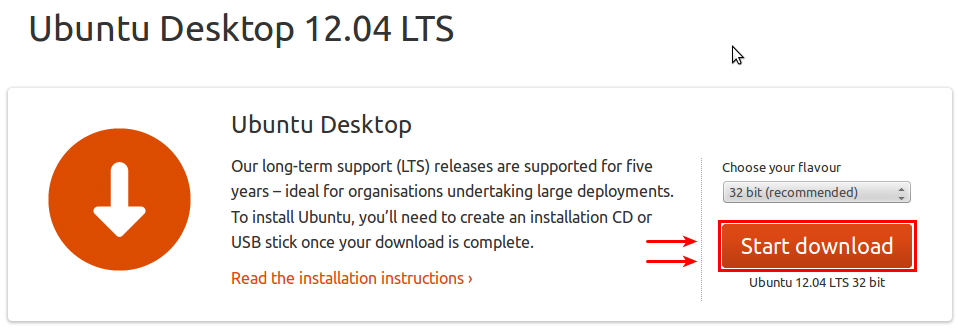
\includegraphics[width=400pt]{./images/obtain-ubuntu/direct-link.png}
	\caption{Direct link download}	
	\label{fig:direct-link}	
	\end{center}
\end{figure}


\subsection*{BitTorrent} \label{sect:obtain_ubuntu_torrent} \index{Download Ubuntu!Torrent}
BitTorrent is a peer-to-peer download network that sometimes enables higher download speeds and more reliable downloads of large files. You will need to install a BitTorrent client on your computer in order to download Ubuntu through this method. You can find all the bittorrent links \href{http://www.ubuntu.com/download/ubuntu/alternative-download}{\textit{here}}.

\subsection*{Buy CDs} \label{sect:obtain_ubuntu_buycd} \index{Download Ubuntu!Buy CD}
If you have a slow internet connection you can always choose to buy the Ubuntu CD and have it shipped to you. However, note that the official CD are only available after a few weeks after a new Ubuntu release. You can buy the CD \href{http://www.ubuntu.com/download/ubuntu/cds}{\textit{here}}. Remember that Ubuntu is completely free. The price covers the production cost of the CDs, excludes applicable VAT, postage and packaging only.

\section{Burning Ubuntu to CD} 
When you download Ubuntu using a direct link or using a torrent as described in section \ref{sect:obtain_ubuntu_direct} and \ref{sect:obtain_ubuntu_torrent}, you finally are presented with a ISO file. Unlike a regular data file, the ISO file cannot be simply dragged and dropped or copied directly onto a disc. It needs to be burned in a specific way that expands/extracts the image so you have usable files on your disc. You can find detailed instructions on how to burn this ISO file into a CD \href{https://help.ubuntu.com/community/BurningIsoHowto}{here} and \href{http://www.ubuntu.com/download/ubuntu/download}{here}. The link provides instruction for Windows and Mac OS users as well.

\section{Create a bootable USB disk} \index{Bootable USB Disk}
In previous chapter you have learned how to make a bootable CD. The story in this section is pretty much the same (actually it's purpose is the same).  The main difference is the media used namely USB stick and BIOS adjustment (removable media has to be on the first place not CD or DVD). If you have a new computer then you might see something like USB CD or DVD  together. In older computers, label in BIOS  is just removable media.  Important to mention, computers that are built before 2001 probably won't have USB listed on a boot device priority. \\

\par \noindent Platform that is going to be used here to make a bootable USB is prior LTS version Ubuntu 10.04 Lucid Lynx. Before you go further be sure that you have USB that holds 2 or more GB of capacity. You can refer \href{http://www.ubuntu.com/download/ubuntu/download}{here} for more information about creating a bootable usb disk for other operating systems.\\

\newpage
\par \noindent Steps to make a bootable USB stick are: \\

\par \noindent 1. Connect your USB to your computer.\\

\par \noindent 2. Run the Startup disk creator application as shown in figure \ref{fig:usb2}. \\

\begin{figure}[h!]	
	\begin{center}
	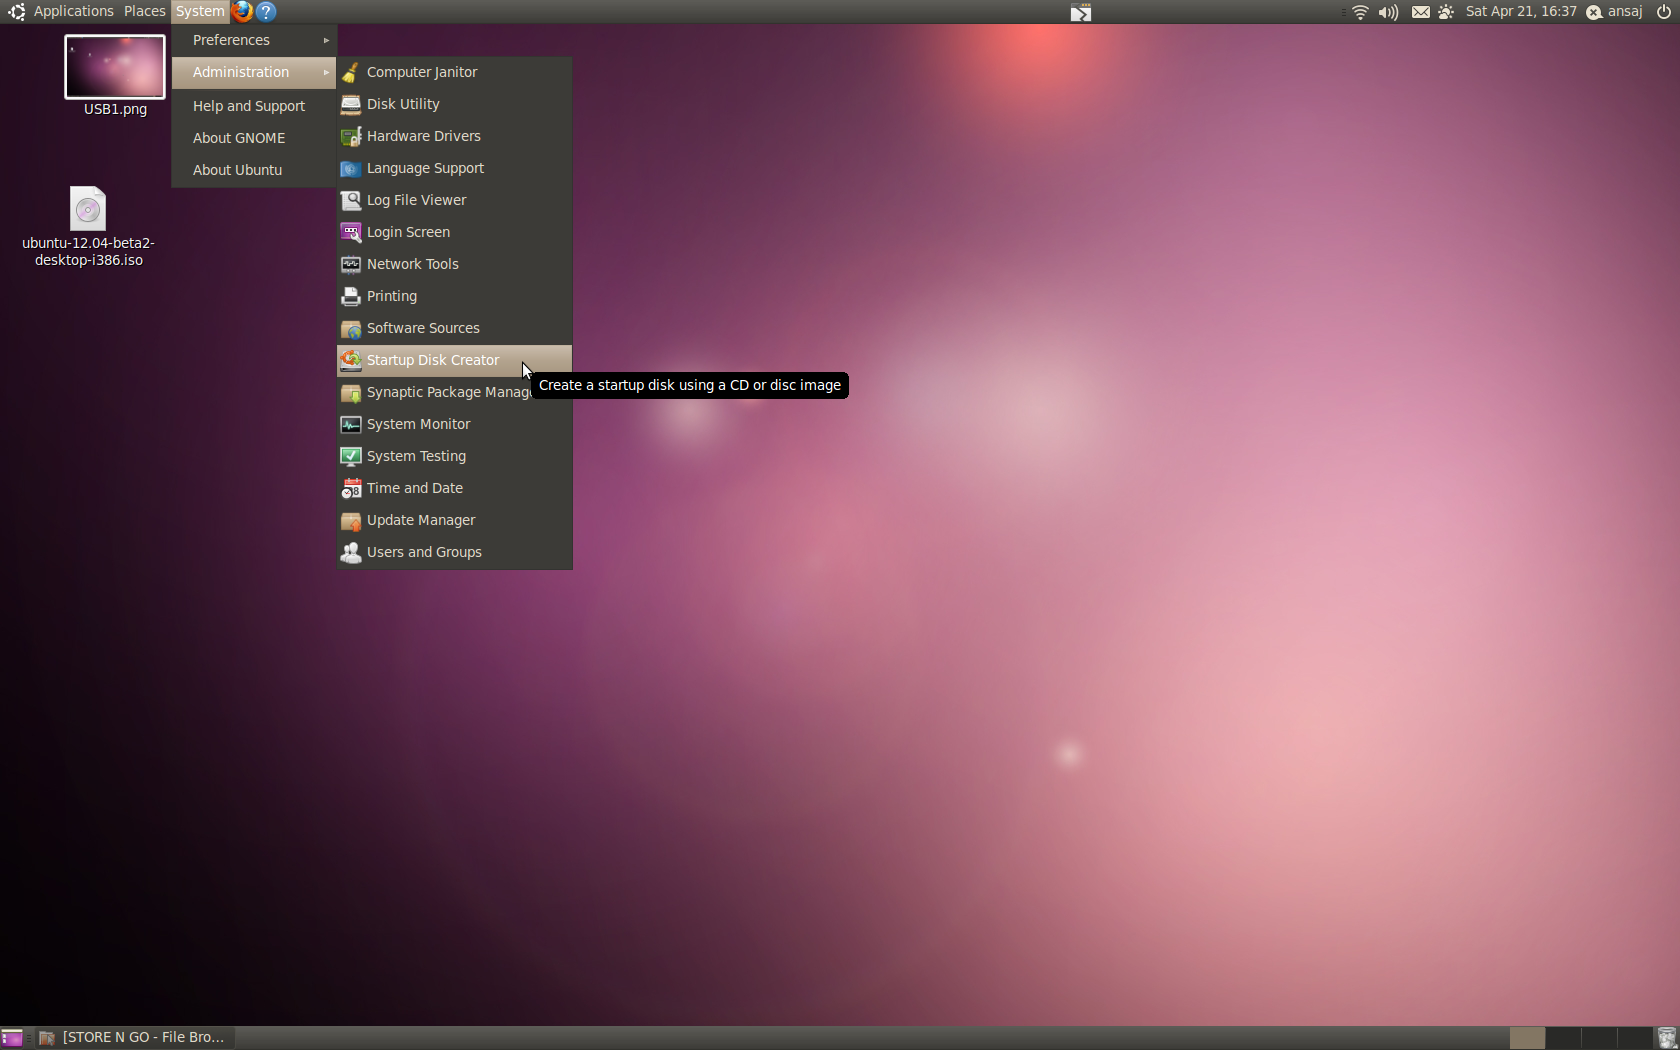
\includegraphics[width=400pt]{./images/obtain-ubuntu/USB2.png}
	\caption{Direct link download}	
	\label{fig:usb2}	
	\end{center}
\end{figure}

\par \noindent 3. After you have started application mentioned in a previous step, you should see something like figure \ref{fig:usb3}. You will notice that application recognized your media (USB) \\

\begin{figure}[h!]	
	\begin{center}
	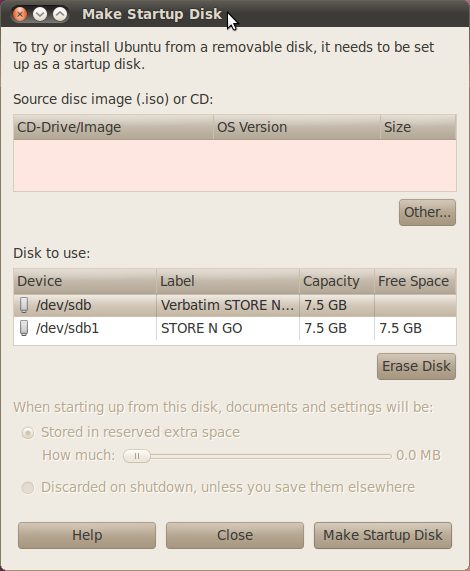
\includegraphics[width=200pt]{./images/obtain-ubuntu/USB3.png}
	\caption{Direct link download}	
	\label{fig:usb3}	
	\end{center}
\end{figure}

\par \noindent 4. Choose your ISO image (depends where you downloaded it or put it). In this example, the ISO is in the desktop. You have to click on the button Other like shown in previous illustration  so you could choose the ISO image. \\

\begin{figure}[h!]	
	\begin{center}
	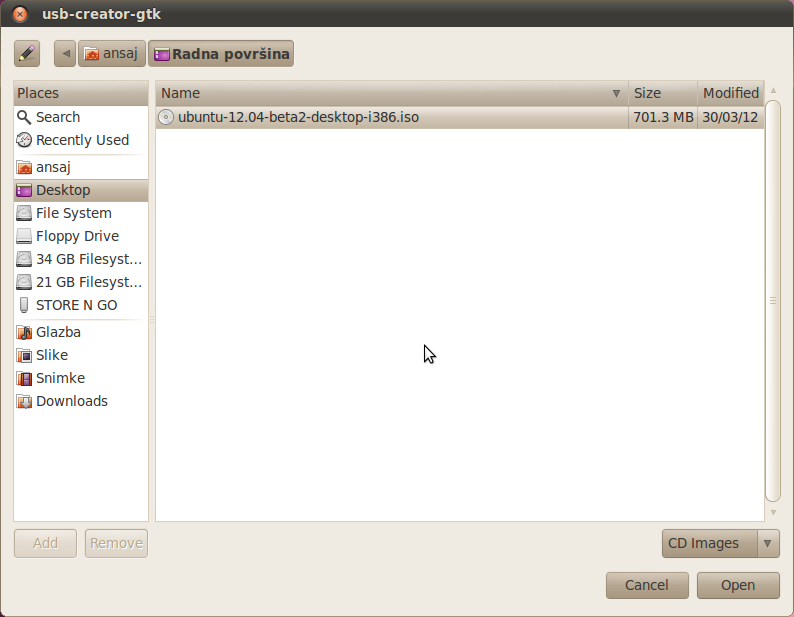
\includegraphics[width=300pt]{./images/obtain-ubuntu/USB4.png}
	\caption{Direct link download}	
	\label{fig:usb4}	
	\end{center}
\end{figure}

\par \noindent 5. After you have chosen the ISO and media, all you have to do is to click on a button  Make startup disk. Don't worry if you are prompted with authentication dialog-box. Just type in your administrator password. Be sure that you do it fast, otherwise you will have to repeat all the steps again. \\

\begin{figure}[h!]	
	\begin{center}
	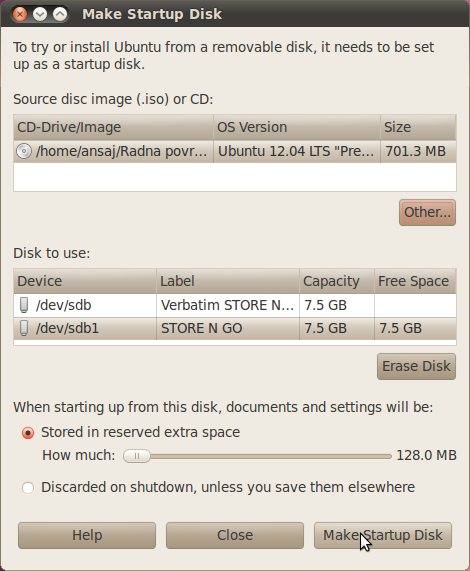
\includegraphics[width=200pt]{./images/obtain-ubuntu/USB6.png}
	\caption{Direct link download}	
	\label{fig:usb6}	
	\end{center}
\end{figure}

\par \noindent Now you will just have to wait until the tool converts your USB into a bootable USB.  After that you can just restart your computer and you are ready to try Ubuntu Live. You can even install it if you know further steps (Installation steps will be shown in the next chapter). Later on, if you decide that  you do not want to have a bootable USB anymore, just format your USB. 